\documentclass[fontset=windows]{article}
\usepackage[margin=1in]{geometry}
\usepackage{ctex}
\usepackage{setspace}
\usepackage{lipsum}
\usepackage{graphicx}
\usepackage{caption}
\usepackage{subcaption}
\usepackage[colorlinks=true,linkcolor=red]{hyperref}

\graphicspath{{figures/}}

\title{\heiti\zihao{2} Common-Source Stage \uppercase\expandafter{\romannumeral1}}
\author{\songti zrrraa}
\date{2023.11.18}

\begin{document}
\maketitle
\thispagestyle{empty}

\section*{CMOS Technology}

\begin{figure}[htbp]
    \centering
    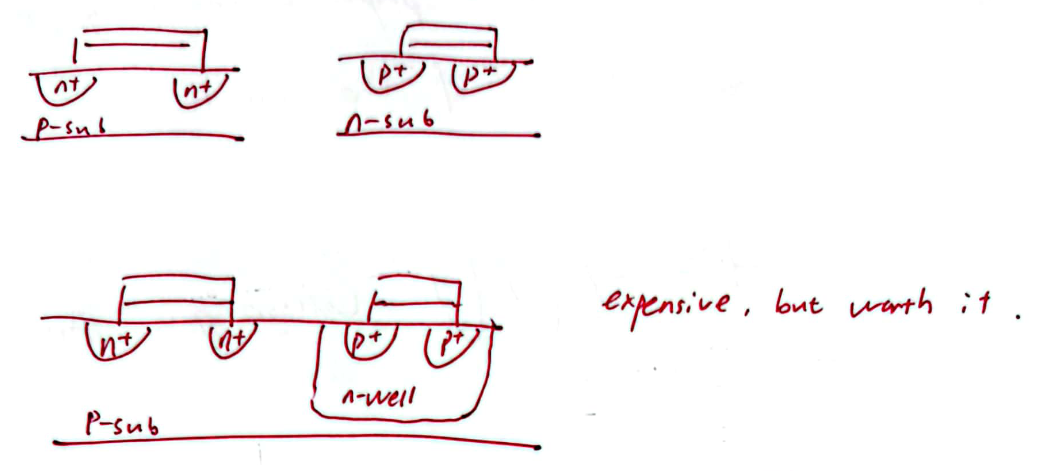
\includegraphics[scale=0.6]{1.jpg}
    \captionsetup{labelformat=empty}
    \caption{}
    \label{1}
\end{figure}

In the 1960s, it was thought that only NMOS would be sufficient because the cost of manufacturing PMOS on a P-type substrate was too high. 
But with the development of the times, people have discovered that the performance of the combination of PMOS and NMOS is very good, 
which cannot be achieved with NMOS alone.

\section*{Judgment of the MOS's working status}

Assume that $V_{THN}=0.5V$, $V_{THP}=-0.6V$. 

\begin{figure}[htbp]
    \centering
    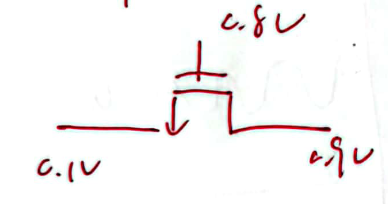
\includegraphics[scale=0.6]{2.jpg}
    \captionsetup{labelformat=empty}
    \caption{}
    \label{2}
\end{figure}

NMOS, $0.8-0.9<0.5$, SAT. 

\begin{figure}[htbp]
    \centering
    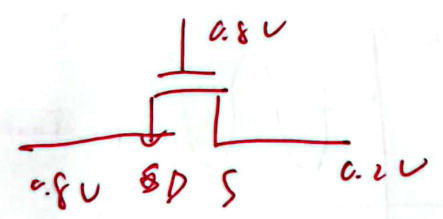
\includegraphics[scale=0.6]{3.jpg}
    \captionsetup{labelformat=empty}
    \caption{}
    \label{3}
\end{figure}

The arrow only indicates the N/PMOS, but not the D/S. 
NMOS has a current flowing from D to S. So here the left is D, the right is S. 

NMOS, $0.8-0.8<0.5$, SAT. 

\begin{figure}[htbp]
    \centering
    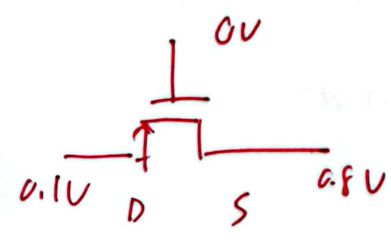
\includegraphics[scale=0.6]{4.jpg}
    \captionsetup{labelformat=empty}
    \caption{}
    \label{4}
\end{figure}

In the same way, this PMOS's left is Drain and the right is Source. 

PMOS, $0.1V-0V<|-0.6V|$, SAT. 

\begin{figure}[htbp]
    \centering
    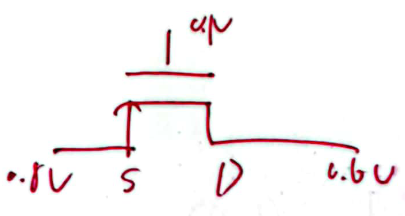
\includegraphics[scale=0.6]{5.jpg}
    \captionsetup{labelformat=empty}
    \caption{}
    \label{5}
\end{figure}

PMOS, $0.6V-0.1V<|-0.6V|$, SAT. 

\section*{CMOS Amplifiers}

\subsection*{Amp design procedure}

\begin{itemize}
    \item select an amp topdogy
    \item Bias the transistor(s) to obtain proper values for $g_m$, $r_o$
    \item Determine the characteristics of the circuit
\end{itemize}

\subsection*{Amp Characteristics}

\begin{itemize}
    \item Gain, usually referred as $A_v$
    \item Power dissipation, etc. 
\end{itemize}

\subsection*{Let's build an amp}

The process is the same as what we talked about before. 

\begin{figure}[htbp]
    \centering
    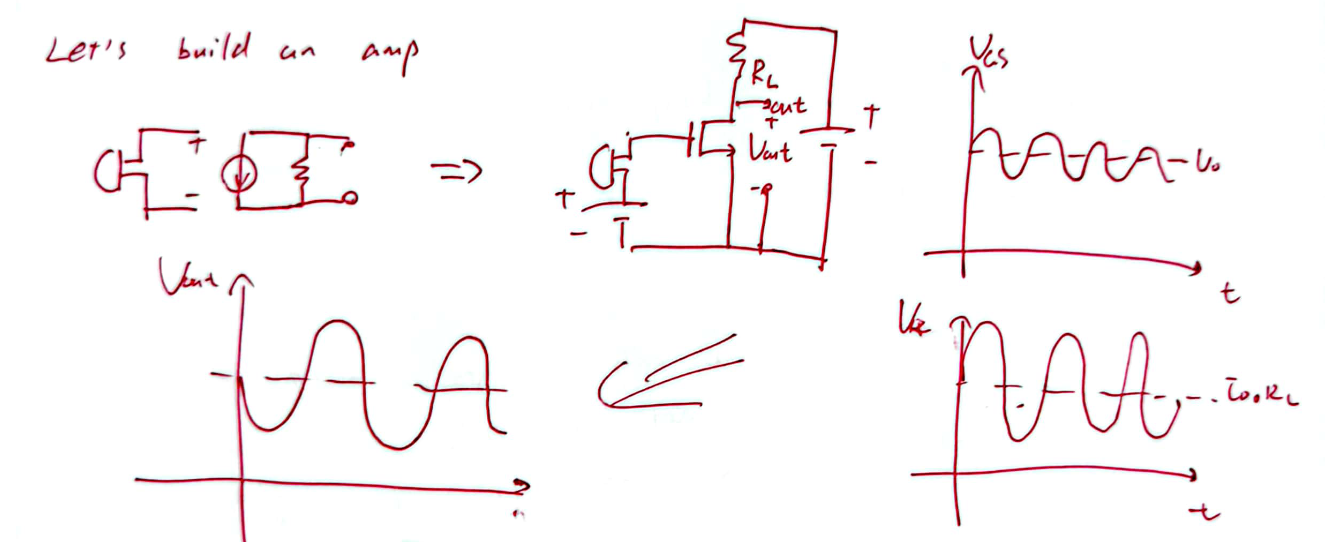
\includegraphics[scale=0.6]{6.jpg}
    \captionsetup{labelformat=empty}
    \caption{}
    \label{6}
\end{figure}

However, here we pick the $V_{DS}$ as the $V_{out}$. This way the amp we build is related to MOS but not the resistor. 

\begin{figure}[htbp]
    \centering
    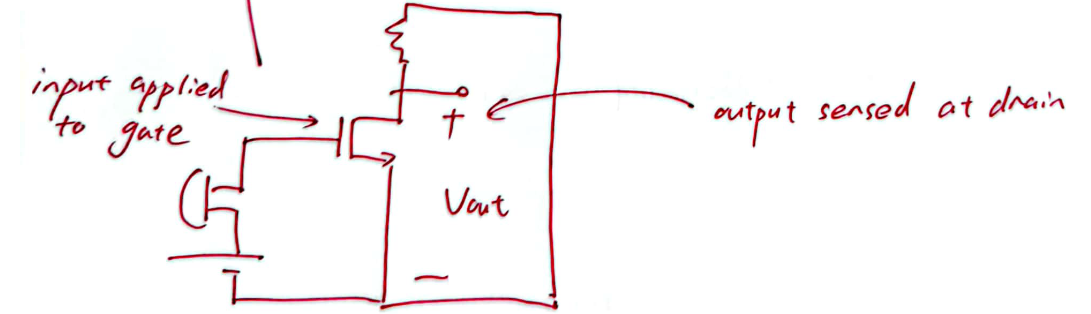
\includegraphics[scale=0.6]{7.jpg}
    \captionsetup{labelformat=empty}
    \caption{}
    \label{7}
\end{figure}

$V_{out}+V_{R_L}=V_2$, So $V_{out}$ is negatively related to the $V_{in}$. 

Let's look at its small-signal model. 

\begin{figure}[htbp]
    \centering
    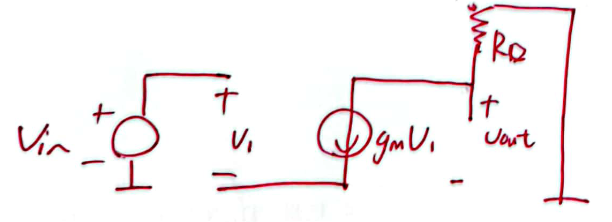
\includegraphics[scale=0.6]{8.jpg}
    \captionsetup{labelformat=empty}
    \caption{The amp's small-signal model}
    \label{8}
\end{figure}

$$V_{in}=V_1$$

$$\frac{V_out}{R_D}+g_mV_1=0$$

In this way we can derive: 

$$\frac{V_{out}}{V_{in}}=-g_mR_D$$

This is called a resistive load common source amplifier. 

\section*{Link}

\href{https://www.bilibili.com/video/BV1FD4y1R7Ah?p=35&vd_source=1d0c07486a3bd3b0adb8ac548bf6453e}{Razavi Electronics Circuits 1: lectrue 35}
\end{document}